\subsection{Normalized Root Mean Square Error (NRMSE)}
We evaluate the NRMSE of our methods to measure the statistical differences between the estimated depths and the depths which were actually observed on October 9th (see section~\ref{realData}). The error along our main interest, the sandbar, is relatively low due to there being less noise within the parameters of the sandbar compared to the error along the 1D transect.
\begin{figure}[H]
		\centering
		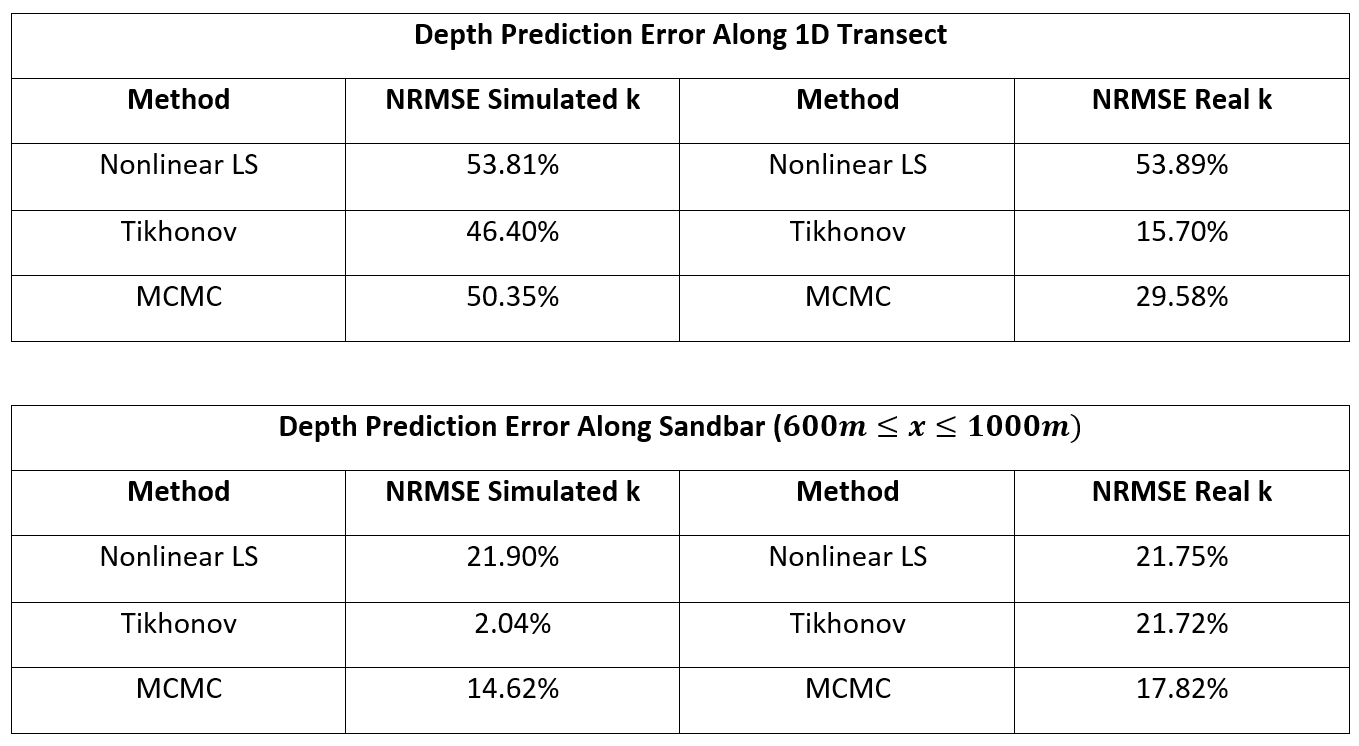
\includegraphics[width=0.80\linewidth]{img/NRMSE_Chart.png}
		\caption{Depth Prediction Error for Estimated Depths}
\end{figure}
		